\chapter{Results}
In order to visually demonstrate the encryption, visualisations of the ciphertext polynomial $c_0$ (refer to \autoref{sec:ckks}) were generated using a CRT decomposition of the RNS representation of $c_0$.
Each pixel corresponds to a coefficient $a \in \Z / q\Z$ scaled down by the modulus $q$ to obtain a brightness value between $0$ and $1$.

\begin{figure}[H]
  \centering
  \pgfplotsset{/pgfplots/group/.cd,vertical sep=1.6cm}
  \inputtikz{figures/generated/training-history}
  \caption{Development of the classification accuracy and the mean squared error during training.}
\end{figure}

\begin{figure}[H]
  \centering
  \inputtikz{figures/generated/confusion-matrix}
  \caption{Confusion Matrix of the trained network.}
\end{figure}

\begin{figure}[H]
  \centering
  % 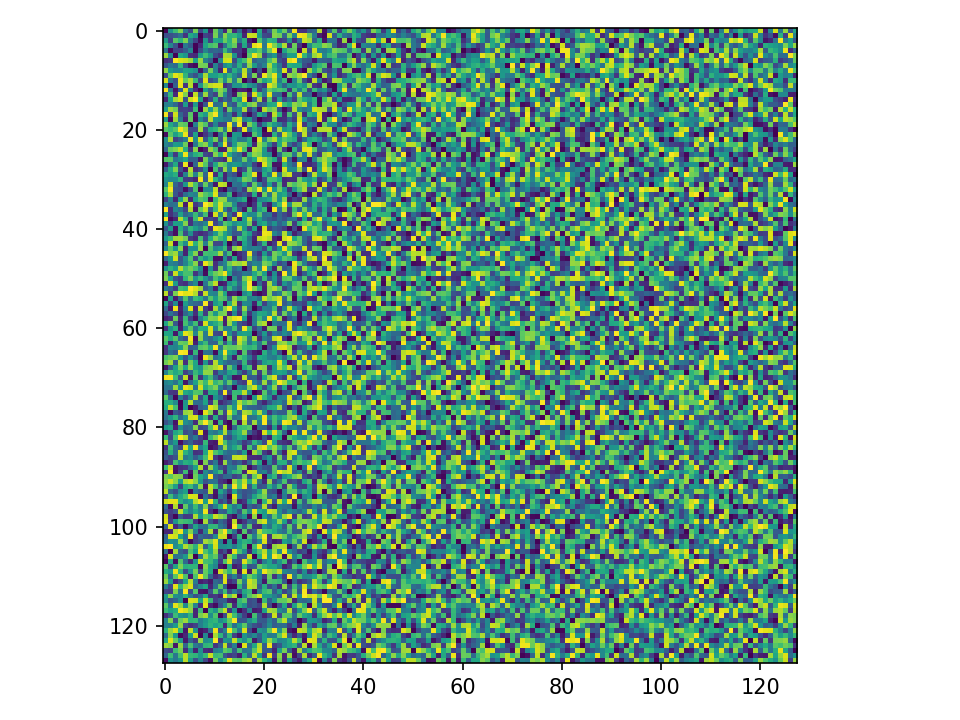
\includegraphics[width=\linewidth]{figures/ciphertext-visualisation.png}
  \inputtikz{figures/ciphertext-visualisation}
  \caption{Ciphertext Visualisation}
\end{figure}

\section{Methodology}
% TODO

\section{Accuracy, Precision, Recall}
The network classifies \SI{97.62}{\percent} of the 10,000 test images correctly.

For a binary classification, two further metrics of interest are
$$\text{Precision} = \frac{\text{tp}}{\text{tp} + \text{fp}} \quad\quad
  \text{Recall} = \frac{\text{tp}}{\text{tp} + \text{fn}}$$

with
$\text{tp}$ ... True Positives,
$\text{fp}$ ... False Positives,
$\text{fn}$ ... False Negatives.

Precision (also referred to as PPV, positive predictive value) refers to the ability of the network to classify positive samples correctly, while Recall explains the completeness of the classified samples (i.e. how few true positives have been left out).

\begin{table}[H]
  \centering
  \caption{Precision and Recall of the trained network for each digit individually}
  \begin{tblr}{r|cccccccccc}
    \textbf{Digit}     & 0     & 1     & 2     & 3     & 4     & 5     & 6     & 7     & 8     & 9     \\
    \hline
    \textbf{Precision} & 0.978 & 0.990 & 0.959 & 0.960 & 0.985 & 0.968 & 0.977 & 0.976 & 0.963 & 0.978 \\
    \textbf{Recall}    & 0.986 & 0.989 & 0.975 & 0.977 & 0.975 & 0.964 & 0.980 & 0.964 & 0.967 & 0.955 \\
  \end{tblr}
\end{table}

Average Precision: \SI{97.37}{\percent} \\
Average Recall: \SI{97.36}{\percent}

\section{Performance Benchmarks}
This chapter includes runtime and communication overhead analysis.

The following benchmarks were accumulated on an Intel \textregistered i7-5600U CPU running at \SI{2.6}{\giga\hertz} as the average over 3 individual runs with different test vectors, consistent accross different parameter runs.

Plain runtime: xxx

\begin{table}[H]
  \centering
  \caption{Performance Benchmarks / Communication Overhead}
  \caption*{
    $B_1$ ... Coefficient Moduli start bits (also equal to the last) \\
    $B_2$ ... Coefficient Moduli middle bits \\
    $N$ ... Polynomial Modulus Degree, found in the exponent of $p(X) = X^N + 1$ \\
    $T$ ... Runtime of encryption, classification, decryption \\
    $M$ ... Message Size \\
    MRE ... Mean Max-Relative Error compared to the exact result, i.e. $\langle \rangle$
  }
  \begin{tblr}{ccrrrrrrl}
    \hline
    \bf SecLevel & \bf MatMul & $\bm{B_1}$ & $\bm{B_2}$ & $\bm{N}$ & $\bm{T}$ / \si{\second} & $\bm{M}$ / \si{\mebi\byte} & \bf MRE / 1 & \bf Mode \\
    \hline
    none         & BSGS       & 34         & 25         & 8192     & 2.9197                  & 132.72                     & 0.13616     & Release  \\
    none         & Hybrid     & 34         & 25         & 8192     & 10.6905                 & 132.72                     & 0.01408     & Release  \\
    none         & BSGS       & 60         & 40         & 16384    & 5.9881                  & 286.50                     & 0.13328     & Release  \\
    none         & Hybrid     & 60         & 40         & 16384    & 19.2554                 & 286.50                     & 0.00185     & Release  \\
    tc128        & BSGS       & 34         & 25         & 8192     & 2.8693                  & 132.72                     & 0.13662     & Release  \\
    tc128        & Hybrid     & 34         & 25         & 8192     & 9.0900                  & 132.72                     & 0.01359     & Release  \\
    tc128        & BSGS       & 60         & 40         & 16384    & 5.9848                  & 286.50                     & 0.13328     & Release  \\
    tc128        & Hybrid     & 60         & 40         & 16384    & 19.0962                 & 286.50                     & 0.00185     & Release  \\
    tc256        & BSGS       & 60         & 40         & 32768    & 13.9787                 & 615.16                     & 0.13328     & Release  \\
    tc256        & Hybrid     & 60         & 40         & 32768    & 41.8026                 & 615.16                     & 0.00185     & Release  \\
    tc128        & BSGS       & 34         & 25         & 8192     & 7.2043                  & 132.72                     & 0.13650     & Debug    \\
    tc128        & Hybrid     & 34         & 25         & 8192     & 13.2971                 & 132.72                     & 0.01369     & Debug    \\
  \end{tblr}
\end{table}

\todo{Multi-row table for better overview?}
